\documentclass[11pt]{article}

\usepackage[margin=1.0in]{geometry}
\usepackage[utf8]{inputenc}
\usepackage[T1]{fontenc}
\usepackage{lmodern}
\usepackage{microtype}
\usepackage{amsmath,amssymb,amsthm}
\usepackage{booktabs}
\usepackage{graphicx}
\usepackage{xcolor}
\usepackage{enumitem}
\usepackage{hyperref}

\hypersetup{
  colorlinks=true,
  linkcolor=blue!60!black,
  citecolor=blue!60!black,
  urlcolor=blue!60!black,
  pdftitle={Certified Optimality and a Spanning-Tree Core Diameter Bound for 2D HP Lattice Protein Folding},
  pdfauthor={Bryan Sanchez},
  pdfsubject={2D HP lattice protein folding, certified global optimality, DRAT and LRAT proofs},
  pdfkeywords={HP lattice protein folding, certified global optimality, Harary-Harborth bound, spanning-tree diameter bound, CP-SAT, DRAT/LRAT proofs}
}

\newtheorem{theorem}{Theorem}
\newtheorem{lemma}{Lemma}

\newcommand{\Z}{\mathbb{Z}}

\title{Certified Optimality and a Spanning-Tree Core Diameter Bound for 2D HP Lattice Protein Folding}

\author{%
  Bryan Sanchez\thanks{%
    Independent Researcher.
    E-mail: \texttt{bryansanchez.bas@gmail.com}.
    ORCID: \href{https://orcid.org/0009-0000-6080-5407}{0009-0000-6080-5407}.}
}

\date{November 26, 2026}

\begin{document}
\maketitle

\begin{abstract}
The two-dimensional hydrophobic--polar (2D HP) lattice protein folding problem is an NP-complete benchmark in combinatorial optimization and statistical physics. Prior exact backtracking established optimal contact counts up to length $85$, yet primary coordinates remained largely unpublished, a four-residue $50$-mer discrepancy persisted, and solver-independent clausal proofs were absent. We make three contributions on $\Z^2$. First, we establish unconditional optimality for S5 ($C^* = 23$) and S9 ($C^* = 53$) analytically via the one-line Harary--Harborth isoperimetric bound, and certify S7 ($C^* = 36$) and S8 ($C^* = 42$) via minimum-perimeter Ferrers enumeration and bipartite parity across four independent solvers (OR-Tools CP-SAT, HiGHS MILP, PicoSAT, and Z3) with six archived DRAT refutation proofs checked by \texttt{drat-trim} and a standalone pure-Python RUP verifier. Second, we prove a spanning-tree core diameter bound valid for disconnected cores---paired with small-component bounds under at most one unit of parity degree slack to cap the component count---certifying $C^*(\mathrm{S6}) = 19$ for the published PP-prefix $50$-mer S6 ($n_H = 22$) across eleven branches via dual-solver refutations and $64.9\,$GB of locally checked LRAT proofs reproducible from archived scripts and verified against an archived SHA-256 ledger (omitted from the repository due to size), resolving the discrepancy with canonical HH-prefix \texttt{2D50} ($C^* = 21$). Third, we print all seven sequences verbatim and archive machine-verified coordinates for S5--S10 and \texttt{2D50}.

\medskip
\noindent\textbf{MSC 2020:} 90C27, 05B50, 92C40, 68T20.

\noindent\textbf{Keywords:} HP lattice protein folding; certified global optimality; Harary--Harborth bound; spanning-tree diameter bound; CP-SAT; DRAT/LRAT proofs.
\end{abstract}

\section{Introduction and Related Work}\label{sec:intro}

In the two-dimensional hydrophobic--polar (HP) lattice model~\cite{dill1985,lau1989}, a protein sequence $s = s_0 s_1 \dots s_{n-1} \in \{\mathrm{H}, \mathrm{P}\}^n$ is embedded as a self-avoiding walk $c = (c_0, \dots, c_{n-1}) \in (\Z^2)^n$ with $\|c_{i+1} - c_i\|_1 = 1$ and $c_i \ne c_j$ ($i \ne j$). The objective is to maximize the count of non-sequential H--H lattice contacts,
\begin{equation}\label{eq:contacts}
  C(c) := \bigl|\bigl\{ (i, j) : 0 \le i < j < n,\; j - i > 1,\; \|c_i - c_j\|_1 = 1,\; s_i = s_j = \mathrm{H} \bigr\}\bigr|.
\end{equation}
Computing $C^*(s) := \max_c C(c)$ is NP-complete in both two dimensions~\cite{crescenzi1998} and three dimensions~\cite{berger1998}. Constant-factor approximation algorithms for the HP model were developed by Hart and Istrail~\cite{hart1996} and improved in 2D by Newman~\cite{newman2002}. A canonical suite of 2D benchmarks of lengths $n \in \{48, 50, 60, 64, 85, 100\}$ (denoted S5--S10 and \texttt{2D50} in Table~\ref{tab:seqs}, originating across~\cite{unger1993,yue1995,beutler1996,ramakrishnan1997,bastolla1998,liang2001,hsu2003,chen2005,zhang2007,wust2012}; in particular, S10 corresponds to the $100$-mer \texttt{2D100b} of Ramakrishnan, Ramachandran, and Pekny~\cite{ramakrishnan1997}) has served as a standard testbed for heuristic and exact methods for more than two decades.

\paragraph{Related exact and heuristic work.}
Exact lattice HP folding methods were pioneered by Yue and Dill's Constrained Hydrophobic Core Construction (CHCC)~\cite{yue1995}, followed by the constraint-based hydrophobic-core-first framework of Will~\cite{will2002}, Backofen and Will~\cite{backofen2006}, and Mann, Will, and Backofen's CPSP-tools~\cite{mann2008} (later coupled with Large Neighborhood Search by Dot\'u, Cebri\'an, Van~Hentenryck, and Clote~\cite{dotu2011}), as well as mixed-integer linear programming formulations on 3D lattices by Yanev, Traykov, Milanov, and Yurukov~\cite{yanev2017}. In 2D, Giaquinta and Pozzi~\cite{giaquinta2013} introduced a sharpened contact upper bound and the specialized exact branch-and-bound algorithm \texttt{minwalk}, establishing optimal contact counts and exact degeneracies for the canonical 2D benchmarks up to length $85$ (including S5 $= 23$, \texttt{2D50} $= 21$, S7 $= 36$, S8 $= 42$, and S9 $= 53$). By contrast, the widely cited branch-and-bound method of Chen and Huang~\cite{chen2005} is an \emph{incomplete heuristic} branch-and-bound algorithm that prunes conformations via a local benefit criterion rather than an admissible bound; crucially, Chen and Huang~\cite[Table~1]{chen2005} also printed the PP-prefix $50$-mer sequence \texttt{PPHPPHPHPHHHHPHPPPHPPPHPPPPHPPPHPPPHPHHHHPHPHPHPHH} ($n_H = 22$, our S6) paired with the target energy $-21$ ($21$ contacts), propagating a benchmark discrepancy relative to Unger and Moult's~\cite{unger1993} canonical HH-prefix \texttt{2D50} sequence ($n_H = 24$, optimal value $21$~\cite{giaquinta2013}).

\paragraph{Comparison with prior exact methods and contributions.}
Compared with specialized exact solvers such as \texttt{minwalk}~\cite{giaquinta2013} and the core-first constraint framework of Backofen and Will~\cite{backofen2006,mann2008}, this work contributes three advances:
\begin{enumerate}[leftmargin=*,topsep=2pt,itemsep=1pt]
\item \emph{Analytic bounds and independent clausal proof certificates across off-the-shelf solvers.} Specialized C/C++ backtracking codes require trusting the correctness of a custom search implementation. Here S5 ($C^* = 23$) and S9 ($C^* = 53$) are established analytically on $\Z^2$ by the one-line Harary--Harborth isoperimetric upper bound matched by verified embeddings, whereas for S7 ($C^* = 36$) and S8 ($C^* = 42$), decoupling minimum-perimeter polyomino enumeration from standard constraint, integer, and propositional solvers---OR-Tools CP-SAT~\cite{perron2023}, HiGHS MILP~\cite{huangfu2018}, PicoSAT~\cite{biere2008}, and Z3~\cite{demoura2008}---certifies unconditional optimality on $\Z^2$ across four independent solvers (combined S7 and S8 model-construction-and-solve times of $0.19\,$s in CP-SAT, $0.45\,$s in HiGHS, and $0.09\,$s in PicoSAT, and $0.91\,$s of Z3 solver-only time, $5.98\,$s end-to-end in Python; Section~\ref{sec:verify}), backed by six archived DRAT refutation proofs checked by \texttt{drat-trim}~\cite{wetzler2014} and a standalone pure-Python RUP verifier.
\item \emph{Exact $\Z^2$ spanning-tree diameter bound for disconnected cores and resolution of the Chen--Huang $50$-mer discrepancy.} Core-first methods~\cite{backofen2006,mann2008} enumerate compact connected H-cores near the isoperimetric ceiling. Because the PP-prefix $50$-mer S6 from~\cite[Table~1]{chen2005} sits $8$ contacts below its Harary--Harborth ceiling ($27$), disconnected H-cores cannot be excluded a priori. Lemma~\ref{lem:spantree} establishes an exact spanning-tree diameter bound over all of $\Z^2$ without assuming core connectivity or an artificial bounding box, paired with small-component bounds under at most one unit of parity degree slack to cap the component count, allowing OR-Tools CP-SAT and CaDiCaL~\cite{biere2024}---together with LRAT clausal proofs~\cite{cruzfilipe2017} checked by \texttt{lrat-check}---to prove $C^*(\mathrm{S6}) = 19$ unconditionally and resolve the $n = 50$ discrepancy.
\item \emph{Verified public coordinate archive.} Major references such as~\cite{wust2012} released explicit coordinates only for $n = 64$, and transcription errors have propagated in derivative studies (for example, identical strings printed for \texttt{2D100a} and \texttt{2D100b} in~\cite{davis2016}). We print all seven sequences verbatim (Table~\ref{tab:seqs}) and archive machine-verified coordinates for S5--S10 and \texttt{2D50}.
\end{enumerate}

\begin{table}[t]
\centering
\caption{Exact benchmark sequences studied in this paper. Underlined colored prefixes highlight the four-residue difference between the PP-prefix variant S6~\cite[Table~1]{chen2005} ($n_H = 22$, $C^* = 19$) and the canonical HH-prefix sequence \texttt{2D50}~\cite{unger1993} ($n_H = 24$, $C^* = 21$~\cite{giaquinta2013}).}
\label{tab:seqs}
\scriptsize
\setlength{\tabcolsep}{3.5pt}
\begin{tabular}{@{}lrl@{}}
\toprule
\textbf{ID} & $n$ & \textbf{Sequence ($s_0 s_1 \dots s_{n-1}$)} \\
\midrule
S5 & 48 & \texttt{PPHPPHHPPHHPPPPPHHHHHHHHHHPPPPPPHHPPHHPPHPPHHHHH} \\
S6 & 50 & \texttt{\textcolor{blue!70!black}{\underline{PPHP}}PHPHPHHHHPHPPPHPPPHPPPPHPPPHPPPHPHHHHPHPHPHPHH} \\
\texttt{2D50} & 50 & \texttt{\textcolor{red!70!black}{\underline{HHPH}}PHPHPHHHHPHPPPHPPPHPPPPHPPPHPPPHPHHHHPHPHPHPHH} \\
S7 & 60 & \texttt{PPHHHPHHHHHHHHPPPHHHHHHHHHHPHPPPHHHHHHHHHHHHPPPPHHHHHHPHHPHP} \\
S8 & 64 & \texttt{HHHHHHHHHHHHPHPHPPHHPPHHPPHPPHHPPHHPPHPPHHPPHHPPHPHPHHHHHHHHHHHH} \\
S9 & 85 & \texttt{HHHHPPPPHHHHHHHHHHHHPPPPPPHHHHHHHHHHHHPPPHHHHHHHHHHHHPPPHHHHHHHHHHHHPPPHPPHHPPHHPPHPH} \\
S10 & 100 & \texttt{PPPHHPPHHHHPPHHHPHHPHHPHHHHPPPPPPPPHHHHHHPPHHHHHHPPPPPPPPPHPHHPHHHHHHHHHHHPPHHHPHHPHPPHPHHHPPPPPPHHH} \\
\bottomrule
\end{tabular}
\end{table}

\section{Analytic Bounds, Spanning-Tree Diameter, and Formal Formulations}\label{sec:methods}

\subsection{Isoperimetric, Parity, and Spanning-Tree Bounds}\label{sec:bounds}

Let $n_H := |\{i : s_i = \mathrm{H}\}|$ be the number of hydrophobic residues and $\mathrm{adj}_{HH} := |\{i : s_i = s_{i+1} = \mathrm{H}\}|$ the number of sequential H--H chain edges. For any finite subset $H \subset \Z^2$ of cardinality $|H| = n_H$, let $\mathrm{ie}(H)$ denote the number of unit lattice edges with both endpoints in $H$, and $P(H) := 4 |H| - 2\,\mathrm{ie}(H)$ its lattice perimeter. Every valid fold $c$ with hydrophobic-site set $H(c) = \{c_i : s_i = \mathrm{H}\}$ satisfies
\begin{equation}\label{eq:ie_rel}
  C(c) = \mathrm{ie}\bigl(H(c)\bigr) - \mathrm{adj}_{HH}.
\end{equation}
For any nonempty finite set $H \subset \Z^2$, define its horizontal and vertical coordinate spans
\[
  \Delta_x(H) := \max_{(x,y)\in H} x - \min_{(x,y)\in H} x,
  \qquad
  \Delta_y(H) := \max_{(x,y)\in H} y - \min_{(x,y)\in H} y,
\]
so that the axis-aligned bounding box of $H$ has width $W(H) := \Delta_x(H) + 1$ and height $B(H) := \Delta_y(H) + 1$.

\begin{lemma}[Harary--Harborth bound and HV-convex minimum-perimeter structure]\label{lem:hh}
For every finite subset $H \subset \Z^2$ with $|H| = m \ge 1$ (connected or disconnected),
\begin{equation}\label{eq:hh}
  \mathrm{ie}(H) \le \mathrm{ie}_{\max}(m) := 2m - \bigl\lceil 2\sqrt{m} \bigr\rceil,
  \qquad\text{equivalently}\qquad
  \frac{P(H)}{2} \ge \bigl\lceil 2\sqrt{m} \bigr\rceil.
\end{equation}
Moreover, if $H$ is connected with bounding-box dimensions $W(H) \times B(H)$ ($W(H) B(H) \ge m$), then $P(H) \ge 2\bigl(W(H) + B(H)\bigr)$ with equality if and only if $H$ is horizontally and vertically convex (HV-convex), in which case its bounding box minus $H$ is a disjoint union of four corner Ferrers diagrams of total area $k = W(H) B(H) - m$.
\end{lemma}

\begin{proof}
For connected $m$-ominoes,~\eqref{eq:hh} is the theorem of Harary and Harborth~\cite{harary1976}. For a disconnected subset $H = H_1 \sqcup \dots \sqcup H_r$ with component sizes $m_1 + \dots + m_r = m$, strict subadditivity of $\sqrt{\cdot}$ gives $\frac{1}{2}P(H) = \sum_{j=1}^r \frac{1}{2}P(H_j) \ge \sum_{j=1}^r \lceil 2\sqrt{m_j}\rceil \ge \lceil 2\sqrt{m}\rceil$. For a connected set $H$, $4$-connectivity guarantees that every column $x \in [x_{\min}(H), x_{\max}(H)]$ and every row $y \in [y_{\min}(H), y_{\max}(H)]$ contains at least one site of $H$. Consequently, each of the $W(H)$ columns contributes at least $2$ horizontal boundary edges (of the unit-square polyomino) and each of the $B(H)$ rows contributes at least $2$ vertical boundary edges, yielding $P(H) \ge 2(W(H) + B(H))$ with equality if and only if every row and every column of $H$ is a single contiguous interval (HV-convexity), leaving four possibly empty corner Ferrers diagrams in the complement inside the bounding box.
\end{proof}

\begin{lemma}[Bipartite checkerboard parity and maximum H-core degree]\label{lem:parity}
Let $s \in \{\mathrm{H}, \mathrm{P}\}^n$ ($n \ge 2$), $E_{\mathrm{seq}} := |\{i \text{ even} : s_i = \mathrm{H}\}|$, and $O_{\mathrm{seq}} := n_H - E_{\mathrm{seq}}$. For each $0 \le i < n$ with $s_i = \mathrm{H}$, define
\[
  d_{\max}(i) := 4 - \mathbf{1}_{i > 0,\, s_{i-1} = \mathrm{P}} - \mathbf{1}_{i < n - 1,\, s_{i+1} = \mathrm{P}} \ge 2.
\]
Then every valid fold $c \in (\Z^2)^n$ with hydrophobic core $H = H(c) = H_{\mathrm{even}} \sqcup H_{\mathrm{odd}}$ (partitioned by $(x + y) \bmod 2$) satisfies
\begin{equation}\label{eq:parity_bal}
  \bigl| |H_{\mathrm{even}}| - |H_{\mathrm{odd}}| \bigr| = |E_{\mathrm{seq}} - O_{\mathrm{seq}}|
\end{equation}
and
\begin{equation}\label{eq:parity_ub}
  C(c) \le \min\!\left(\sum_{i \text{ even},\, s_i=\mathrm{H}} d_{\max}(i),\; \sum_{i \text{ odd},\, s_i=\mathrm{H}} d_{\max}(i)\right) - \mathrm{adj}_{HH}.
\end{equation}
\end{lemma}

\begin{proof}
Because every unit step changes $(x + y) \bmod 2$ by $1$, the checkerboard parity of $c_i$ is fixed by $i \bmod 2$ up to a single global shift $\pi \in \{0, 1\}$, immediately yielding~\eqref{eq:parity_bal}. Each hydrophobic residue $s_i = \mathrm{H}$ has $4$ lattice neighbors, losing one available H-core neighbor for each adjacent polar residue along the chain (an endpoint $i \in \{0, n - 1\}$ has only one chain neighbor, so $d_{\max}(i) \in \{3, 4\}$, while an internal H residue has $d_{\max}(i) \in \{2, 3, 4\}$). Thus $\deg_H(c_i) \le d_{\max}(i)$ for every H residue. Since $\Z^2$ is bipartite, every internal edge of $H$ joins one even-indexed H residue to one odd-indexed H residue, so $\mathrm{ie}(H) = \sum_{i \text{ even},\, s_i=\mathrm{H}} \deg_H(c_i) = \sum_{i \text{ odd},\, s_i=\mathrm{H}} \deg_H(c_i)$. Substituting into~\eqref{eq:ie_rel} yields~\eqref{eq:parity_ub}.
\end{proof}

When the contact gap to the Harary--Harborth ceiling is large (as on S6, where $C \le 21 < 27$), disconnected hydrophobic cores $H = H_1 \sqcup \dots \sqcup H_r$ cannot be excluded a priori. The following lemma provides an exact bounding-box diameter bound over \emph{all} of $\Z^2$ that remains valid for disconnected cores.

\begin{lemma}[Exact spanning-tree H-core diameter bound over all of $\Z^2$]\label{lem:spantree}
Let $c \in (\Z^2)^n$ ($n \ge 2$) be any self-avoiding walk of $s$ with hydrophobic core $H = H(c) = H_1 \sqcup \dots \sqcup H_r$ decomposed into its $r \ge 1$ lattice-connected ($4$-connected) components of sizes $v_1 + \dots + v_r = n_H$. Let $g_1 \ge g_2 \ge \dots \ge g_{n_H - 1}$ be the consecutive H-to-H chain index gaps sorted in nonincreasing order, define the parity degree slacks
\[
  s_{\mathrm{odd}} := \sum_{i \text{ odd},\, s_i=\mathrm{H}} d_{\max}(i) - \mathrm{ie}(H) \ge 0,
  \qquad
  s_{\mathrm{even}} := \sum_{i \text{ even},\, s_i=\mathrm{H}} d_{\max}(i) - \mathrm{ie}(H) \ge 0,
\]
and set $s_{\min} := \min(s_{\mathrm{odd}}, s_{\mathrm{even}})$ and $s_{\max} := \max(s_{\mathrm{odd}}, s_{\mathrm{even}})$. Then:
\begin{enumerate}[leftmargin=*,topsep=2pt,itemsep=1pt]
\item \emph{(Spanning-tree bounding-box inequality.)}
\begin{equation}\label{eq:spantree}
  \Delta_x(H) + \Delta_y(H) \le \frac{P(H)}{2} - 2r + \sum_{m=1}^{r-1} g_m.
\end{equation}
\item \emph{(Slack constraints on small components.)} Let $c_1 := |\{j : v_j = 1\}|$ and $c_2 := |\{j : v_j = 2\}|$. Whenever $s_{\min} \le 1$, we have
\begin{equation}\label{eq:smallcomp}
  c_2 \le s_{\min},
  \qquad
  2 c_1 + c_2 \le s_{\max},
  \qquad
  \sum_{j=1}^r \bigl\lceil 2\sqrt{v_j} \bigr\rceil \le \frac{P(H)}{2}.
\end{equation}
\item \emph{(Exact evaluation for S6.)} For the PP-prefix sequence S6 ($n_H = 22$, $\mathrm{adj}_{HH} = 7$, $\sum_{\mathrm{odd}} d_{\max} = 28$, $\sum_{\mathrm{even}} d_{\max} = 31$, sorted H-to-H gaps $(5, 4, 4, 4, 4, 3, 2, \dots)$):
\begin{align*}
  C(c) = 21 &\implies r \le 3,\quad \Delta_x(H) + \Delta_y(H) \le 19, \\
  C(c) = 20 &\implies r \le 4,\quad \Delta_x(H) + \Delta_y(H) \le 22.
\end{align*}
\end{enumerate}
\end{lemma}

\begin{proof}
\textbf{(1)} By Lemma~\ref{lem:hh}, each connected component $H_j$ satisfies $W(H_j) + B(H_j) \le P(H_j)/2$, so $\Delta_x(H_j) + \Delta_y(H_j) \le P(H_j)/2 - 2$. Contracting each component $H_j$ to a single vertex produces a connected multigraph on $\{1, \dots, r\}$ whose edges correspond to consecutive H-to-H chain subsegments of lengths $g_m$. Select any spanning tree $T$ of this multigraph ($r - 1$ distinct chain gaps). Each tree edge $e \in T$ joins some $u_e \in H_a$ and $v_e \in H_b$ along a chain subsegment of length $g(e)$, so $|\Delta x(e)| + |\Delta y(e)| = \|u_e - v_e\|_1 \le g(e)$. Let $x_{\min}(H), x_{\max}(H)$ be attained in components $H_{a_1}, H_{a_2}$ and $y_{\min}(H), y_{\max}(H)$ in $H_{b_1}, H_{b_2}$. Traversing the unique simple path in $T$ from $H_{a_1}$ to $H_{a_2}$ visits each component and each tree edge at most once, giving $\Delta_x(H) \le \sum_{j=1}^r \Delta_x(H_j) + \sum_{e \in T} |\Delta x(e)|$. Adding the analogous bound for $\Delta_y(H)$ yields
\[
  \Delta_x(H) + \Delta_y(H)
  \le \sum_{j=1}^r \left(\frac{P(H_j)}{2} - 2\right) + \sum_{e \in T} \bigl(|\Delta x(e)| + |\Delta y(e)|\bigr)
  \le \frac{P(H)}{2} - 2r + \sum_{m=1}^{r-1} g_m.
\]

\textbf{(2)} Without loss of generality, let the parity class attaining $s_{\min}$ be the odd-indexed H residues (the even case is identical by symmetry). By Lemma~\ref{lem:parity}, every H residue satisfies $d_{\max}(i) \ge 2$. When $s_{\min} \le 1$, every odd H residue has $\deg_H(c_i) \ge d_{\max}(i) - s_{\min} \ge 1$, so no odd H residue can form an isolated component ($v_j = 1$). Every size-$1$ component is therefore an isolated even H residue (degree $0$), consuming $d_{\max}(i) \ge 2$ units of $s_{\max}$. Every size-$2$ component is a single bipartite edge between one odd H and one even H of degree $1$ each, consuming at least $1$ unit of $s_{\min}$ and at least $1$ unit of $s_{\max}$. Summing over all components gives $c_2 \le s_{\min}$ and $2c_1 + c_2 \le s_{\max}$, while Lemma~\ref{lem:hh} gives $\sum_{j=1}^r \lceil 2\sqrt{v_j}\rceil \le \sum_{j=1}^r P(H_j)/2 = P(H)/2$.

\textbf{(3)} For S6 (Table~\ref{tab:seqs}), the $22$ hydrophobic indices are
\[
  \{2, 5, 7, 9, 10, 11, 12, 14, 18, 22, 27, 31, 35, 37, 38, 39, 40, 42, 44, 46, 48, 49\},
\]
whose consecutive gaps in nonincreasing order begin $(5, 4, 4, 4, 4, 3, 2, \dots)$. Since $\sum_{j=1}^r \lceil 2\sqrt{v_j}\rceil \ge \sum_{j=1}^r 2\sqrt{v_j}$ and $v \mapsto 2\sqrt{v}$ is strictly concave and strictly subadditive, for fixed $(r, c_1, c_2)$ the continuous sum $\sum_{j=1}^r 2\sqrt{v_j}$ is minimized by setting $r - 1 - c_1 - c_2$ parts equal to $3$ and concentrating the remaining mass in one largest part $M \ge 3$:
\begin{itemize}[leftmargin=*,topsep=1pt,itemsep=1pt]
\item At $C = 21$: $\mathrm{ie}(H) = 28$, $P(H)/2 = 16$, $s_{\min} = s_{\mathrm{odd}} = 0$, and $s_{\max} = s_{\mathrm{even}} = 3$, forcing $c_2 = 0$ and $c_1 \le 1$. Since $c_1 + c_2 \le 1$, any partition with $r \ge 4$ has at least $r - 1 \ge 3$ parts of size at least $3$; repeatedly merging two parts of size at least $3$ reduces $r$ to $4$ while preserving $(c_1, c_2)$ and strictly decreasing $\sum 2\sqrt{v_j}$. At $r = 4$, the continuous lower bound is minimized at $(15, 3, 3, 1)$ with $2\sqrt{15} + 4\sqrt{3} + 2 \approx 16.674 > 16$ (and at $(13, 3, 3, 3)$ for $c_1 = 0$, giving $17.603 > 16$; exhaustive integer enumeration gives exact minima $18$ and $19$). Hence $r \le 3$, and~\eqref{eq:spantree} is maximized at $r = 3$ (feasible via $(18, 3, 1)$ with perimeter sum $9 + 4 + 2 = 15 \le 16$), giving $\Delta_x(H) + \Delta_y(H) \le 16 - 2(3) + (5 + 4) = 19$.
\item At $C = 20$: $\mathrm{ie}(H) = 27$, $P(H)/2 = 17$, $s_{\min} = s_{\mathrm{odd}} = 1$, and $s_{\max} = s_{\mathrm{even}} = 4$, forcing $c_2 \le 1$ and $2c_1 + c_2 \le 4$. The five allowed pairs are $(c_1, c_2) \in \{(2, 0), (1, 1), (1, 0), (0, 1), (0, 0)\}$, all satisfying $c_1 + c_2 \le 2$. Thus any partition with $r \ge 5$ has at least $r - 2 \ge 3$ parts of size at least $3$; merging two such parts reduces $r$ to $5$ while preserving $(c_1, c_2)$ and strictly decreasing $\sum 2\sqrt{v_j}$. At $r = 5$, the continuous concave lower bounds across the five pairs are $2\sqrt{14} + 4\sqrt{3} + 4 \approx 18.41$, $2\sqrt{13} + 4\sqrt{3} + 2\sqrt{2} + 2 \approx 18.97$, $2\sqrt{12} + 6\sqrt{3} + 2 \approx 19.32$, $2\sqrt{11} + 6\sqrt{3} + 2\sqrt{2} \approx 19.85$, and $2\sqrt{10} + 8\sqrt{3} \approx 20.18$, all strictly greater than $17$ (exhaustive integer enumeration yields exact integer minima $19, 20, 20, 21, 21$, attained by $(12, 4, 4, 1, 1)$, $(9, 6, 4, 2, 1)$, $(9, 4, 4, 4, 1)$, $(6, 6, 4, 4, 2)$, and $(6, 4, 4, 4, 4)$). Hence $r \le 4$, and~\eqref{eq:spantree} is maximized at $r = 4$ (feasible via $(16, 4, 1, 1)$ with perimeter sum $8 + 4 + 2 + 2 = 16 \le 17$), giving $\Delta_x(H) + \Delta_y(H) \le 17 - 2(4) + (5 + 4 + 4) = 22$.
\end{itemize}
Both bounds are additionally confirmed by exhaustive enumeration over all $1{,}002$ integer partitions of $22$.
\end{proof}

\subsection{Unconditional Padding and Formal Solver Formulations}\label{sec:formulations}

Given a fixed target hydrophobic core $H \subset \Z^2$ with $|H| = n_H$, any polar residue $s_i = \mathrm{P}$ belonging to a maximal contiguous P-run of length $L$ lies at lattice Manhattan distance at most $\lceil L/2 \rceil$ from $H$ if flanked by H residues on both sides, and at most $L$ if it lies in a terminal P-run. Consequently, padding the axis-aligned bounding box of $H$ on all four sides by $\mathrm{pad} = L_{\max} + 1$ (where $L_{\max}$ is the maximum contiguous P-run length in $s$) yields a finite grid $\mathcal{G} \subset \Z^2$ containing \emph{every} valid embedding of $s$ in $\Z^2$ with hydrophobic core $H$, without loss of generality. Let $P_{\mathcal{G}} := \mathcal{G} \setminus H$ and let $N(u) := \{v \in \Z^2 : \|u - v\|_1 = 1\}$ denote the four lattice neighbors of $u$. We cross-verify fixed-core routability and free-core S6 feasibility using three independent mathematical formulations:

\begin{enumerate}[leftmargin=*,topsep=2pt,itemsep=2pt]
\item \emph{CP-SAT integer cell-ID model (fixed-core routability).} Index $\mathcal{G}$ bijectively by $\{0, \dots, |\mathcal{G}| - 1\}$, and introduce an integer variable $x_i$ for each residue $0 \le i < n$ with domain $x_i \in H$ if $s_i = \mathrm{H}$ and $x_i \in P_{\mathcal{G}}$ if $s_i = \mathrm{P}$. Enforce self-avoidance via $\mathrm{AllDifferent}(x_0, \dots, x_{n-1})$ and chain continuity via allowed-assignment table constraints $(x_i, x_{i+1}) \in E(\mathcal{G})$ for $0 \le i < n - 1$, where $E(\mathcal{G}) := \{(u, v) \in \mathcal{G}^2 : \|u - v\|_1 = 1\}$. Because $|H| = n_H$ and the variables are pairwise distinct, every site of $H$ is automatically covered by an H residue. No residue-level symmetry breaking is imposed.

\item \emph{MILP binary occupancy model (fixed-core routability and free-core S6).} For fixed-core routability under checkerboard parity offset $\pi \in \{0, 1\}$, restrict residue $i$ to parity-compatible sites $V_i := \{u \in \mathcal{D}_i : (u_x + u_y) \equiv i + \pi \pmod 2\}$ (with $\mathcal{D}_i = H$ if $s_i = \mathrm{H}$ and $P_{\mathcal{G}}$ otherwise) and introduce binary occupancy indicators $p_{i,u} \in \{0, 1\}$ for $u \in V_i$:
\begin{equation}\label{eq:milp_core}
\begin{gathered}
  \sum_{u \in V_i} p_{i,u} = 1 \;\; (\forall i),
  \qquad\qquad
  \sum_{i : u \in V_i} p_{i,u} \begin{cases} = 1, & u \in H, \\ \le 1, & u \in P_{\mathcal{G}}, \end{cases} \\[3pt]
  p_{i,u} \le \sum_{v \in N(u) \cap V_{i+1}} p_{i+1,v} \quad (\forall i < n - 1,\; u \in V_i).
\end{gathered}
\end{equation}
For the free-core S6 problem (solved in binary-occupancy CP-SAT and cross-checked in HiGHS MILP), $V_i$ is the exact finite diamond of Cut~2 (Section~\ref{sec:s6}), and we add H-occupancy bits $h_u = \sum_{i : s_i=\mathrm{H},\, u \in V_i} p_{i,u} \in \{0, 1\}$, bipartite H--H edge indicators $z_{uv} \in \{0, 1\}$ for adjacent odd--even pairs $(u, v)$ satisfying $z_{uv} \le h_u$ and $z_{uv} \le h_v$ (plus $z_{uv} \ge h_u + h_v - 1$ in the exact HiGHS feasibility check), bounding-box extent variables $x_{\min}, x_{\max}, y_{\min}, y_{\max}$ coupled to $h_u$ via $(x_{\max} - x_{\min}) + (y_{\max} - y_{\min}) \le D$, and exact degree equations on odd H sites and upper degree bounds on even H sites.

\item \emph{Pure-Boolean CNF encodings and sound S6 relaxation.} For fixed-core routability (PicoSAT and Z3 DRAT generation), the variables $p_{i,u}$ in~\eqref{eq:milp_core} are encoded in pure propositional CNF using Sinz's linear-size sequential counter~\cite{sinz2005} for every $\mathrm{AtMostOne}$ constraint of cardinality $> 4$ (pairwise clauses for cardinality $\le 4$), together with bidirectional adjacency clauses $\neg p_{i,u} \vee \bigvee_{v \in N(u) \cap V_{i+1}} p_{i+1,v}$ and $\neg p_{i+1,v} \vee \bigvee_{u \in N(v) \cap V_i} p_{i,u}$. For the free-core S6 refutations in CaDiCaL/LRAT, let $V_{\mathrm{H}} := \bigcup_{j : s_j = \mathrm{H}} V_j$ denote the set of H-admissible lattice sites, and for each odd H residue $i \in \{5, 7, 9, 11, 27, 31, 35, 37, 39, 49\}$ let $r_i := d_{\max}(i) - \sigma_i \in \{1, 2, 3, 4\}$ denote its required H-core degree in the given odd-H slack branch (with slack $\sigma_i \in \{0, 1\}$ as defined in Cut~4, Section~\ref{sec:s6}). We encode $p_{i,u}$, $h_u \iff \bigvee_{i : s_i=\mathrm{H},\, u \in V_i} p_{i,u}$, the Cut~1 inequality $\Delta_x(H) + \Delta_y(H) \le D$ via a monotone unary order encoding of the four bounding-box extremes and their $x$- and $y$-spans, Cut~3's upper cap $\deg_H(\mathrm{H}_2) \le 2$ (forbidding every triple of H-occupied neighbors around $\mathrm{H}_2$), and the odd-H degree lower bounds $\deg_H(c_i) \ge r_i$ across all $10$ odd H residues: for each candidate cell $u \in V_i$, setting $m := |N(u) \cap V_{\mathrm{H}}|$, we add the unit-forbidding clause $\neg p_{i,u}$ whenever $m < r_i$, and otherwise add the $\binom{m}{m - r_i + 1}$ neighborhood clauses $\neg p_{i,u} \vee \bigvee_{v \in S} h_v$ over all subsets $S \subseteq N(u) \cap V_{\mathrm{H}}$ of size $m - r_i + 1$. Crucially, whereas the CP-SAT model retains edge variables $z_{uv}$ for Cut~4 and adds Cut~5's direct neighbor-forcing valid inequalities only for the five $d_{\max} \in \{3, 4\}$ odd H residues $\{9, 11, 37, 39, 49\}$, this pure-CNF formula omits $z_{uv}$ and the upper degree bounds on even H residues other than $\mathrm{H}_2$, enforcing the neighborhood lower-bound clauses on all $10$ odd H residues instead. Because every valid fold of S6 achieving contact count $C$ in a given odd-H slack branch satisfies $\deg_H(c_i) = r_i$ (hence $\deg_H(c_i) \ge r_i$) at every odd H residue, $\deg_H(\mathrm{H}_2) \le 2$, and $\Delta_x(H) + \Delta_y(H) \le D$, omitting $z_{uv}$ and the remaining even-H upper bounds yields a relaxation (a superset of the feasible set); thus the pure-CNF encoding is a \emph{sound relaxation} for proving unsatisfiability, and any LRAT refutation rules out all valid folds in that branch unconditionally.
\end{enumerate}

\section{Global Optimality Certification for S5, S7, S8, and S9}\label{sec:opt}

\begin{theorem}[Unconditional global optimality on $\Z^2$ for S5, S7, S8, and S9]\label{thm:opt}
Confirming the optimal contact counts established via \textup{\texttt{minwalk}} in~\cite{giaquinta2013}, over all self-avoiding walks in $\Z^2$ (allowing connected or disconnected hydrophobic cores):
\begin{enumerate}[leftmargin=*,topsep=2pt,itemsep=1pt]
\item $C^*(\mathrm{S5}) = 23$ ($n = 48$, $n_H = 25$, $\mathrm{adj}_{HH} = 17$);
\item $C^*(\mathrm{S7}) = 36$ ($n = 60$, $n_H = 43$, $\mathrm{adj}_{HH} = 35$);
\item $C^*(\mathrm{S8}) = 42$ ($n = 64$, $n_H = 42$, $\mathrm{adj}_{HH} = 28$);
\item $C^*(\mathrm{S9}) = 53$ ($n = 85$, $n_H = 59$, $\mathrm{adj}_{HH} = 49$).
\end{enumerate}
\end{theorem}

\begin{proof}
\textbf{Lower bounds.} Direct coordinate verification confirms that our archived lattice embeddings for S5, S7, S8, and S9 are valid self-avoiding walks attaining $23, 36, 42$, and $53$ non-sequential H--H contacts, respectively (Figure~\ref{fig:gallery}).

\textbf{Upper bounds for S5 and S9.} By Lemma~\ref{lem:hh} and~\eqref{eq:ie_rel}:
\begin{align*}
  \mathrm{S5}:&\quad \mathrm{ie}_{\max}(25) = 50 - \lceil 2\sqrt{25}\rceil = 40 \implies C(\mathrm{S5}) \le 40 - 17 = 23, \\
  \mathrm{S9}:&\quad \mathrm{ie}_{\max}(59) = 118 - \lceil 2\sqrt{59}\rceil = 102 \implies C(\mathrm{S9}) \le 102 - 49 = 53.
\end{align*}

\textbf{Upper bound for S8 ($C \le 42$).} Attaining $C \ge 43$ requires $\mathrm{ie}(H) \ge 43 + 28 = 71 = \mathrm{ie}_{\max}(42)$, i.e., $P(H)/2 \le 13$. If $H$ were disconnected ($r \ge 2$), taking $A$ to be a smallest connected component ($1 \le a := |A| \le 21$) and $b := 42 - a$ would give $P(H)/2 \ge \lceil 2\sqrt{a}\rceil + \lceil 2\sqrt{b}\rceil \ge 15 > 13$ for every $1 \le a \le 21$; hence $H$ must be connected. Since $W + B \le 12 \implies W B \le 36 < 42$, every achieving connected $42$-omino satisfies $W + B = 13 = P(H)/2$ and is HV-convex with unique integer box $\{W, B\} = \{6, 7\}$ ($k = 42 - 42 = 0$). Thus the \emph{unique} $42$-cell subset of $\Z^2$ (up to $D_4$ isometry) with $\mathrm{ie}(H) \ge 71$ is the $6 \times 7$ rectangle. Because S8 has longest P-run $L_{\max} = 2$, padding $\mathrm{pad} = 3$ is unconditional over $\Z^2$. Both checkerboard parity alignments of the $6 \times 7$ rectangle are certified unroutable by the independent solvers and machine-checked DRAT proofs detailed in Section~\ref{sec:verify}.

\textbf{Upper bound for S7 ($C \le 36$).} Attaining $C \ge 37$ requires $\mathrm{ie}(H) \ge 37 + 35 = 72 = \mathrm{ie}_{\max}(43)$, i.e., $P(H)/2 \le 14$. If $H$ were disconnected, taking $A$ to be a smallest connected component ($1 \le a := |A| \le 21$) and $b := 43 - a$ would give $P(H)/2 \ge \lceil 2\sqrt{a}\rceil + \lceil 2\sqrt{b}\rceil \ge 15 > 14$, so $H$ must be connected. Since $W + B \le 13 \implies W B \le 42 < 43$, every achieving $43$-omino is HV-convex with $W + B = 14$ and $W B \ge 43$, i.e., $\{W, B\} \in \{\{5, 9\}, \{6, 8\}, \{7, 7\}\}$. Exhaustive four-corner Ferrers enumeration yields exactly $147$ canonical $43$-ominoes with $\mathrm{ie}(H) \ge 72$. For S7, $E_{\mathrm{seq}} = 23$ and $O_{\mathrm{seq}} = 20$, so~\eqref{eq:parity_bal} requires $\bigl||H_{\mathrm{even}}| - |H_{\mathrm{odd}}|\bigr| = 3$, filtering the $147$ candidates to exactly $4$ shapes. Because S7 has $L_{\max} = 4$, padding $\mathrm{pad} = 5$ is unconditional over $\Z^2$. All four surviving shapes are certified unroutable by the independent solvers and machine-checked DRAT proofs detailed in Section~\ref{sec:verify}.
\end{proof}

\begin{figure}[tb]
\centering
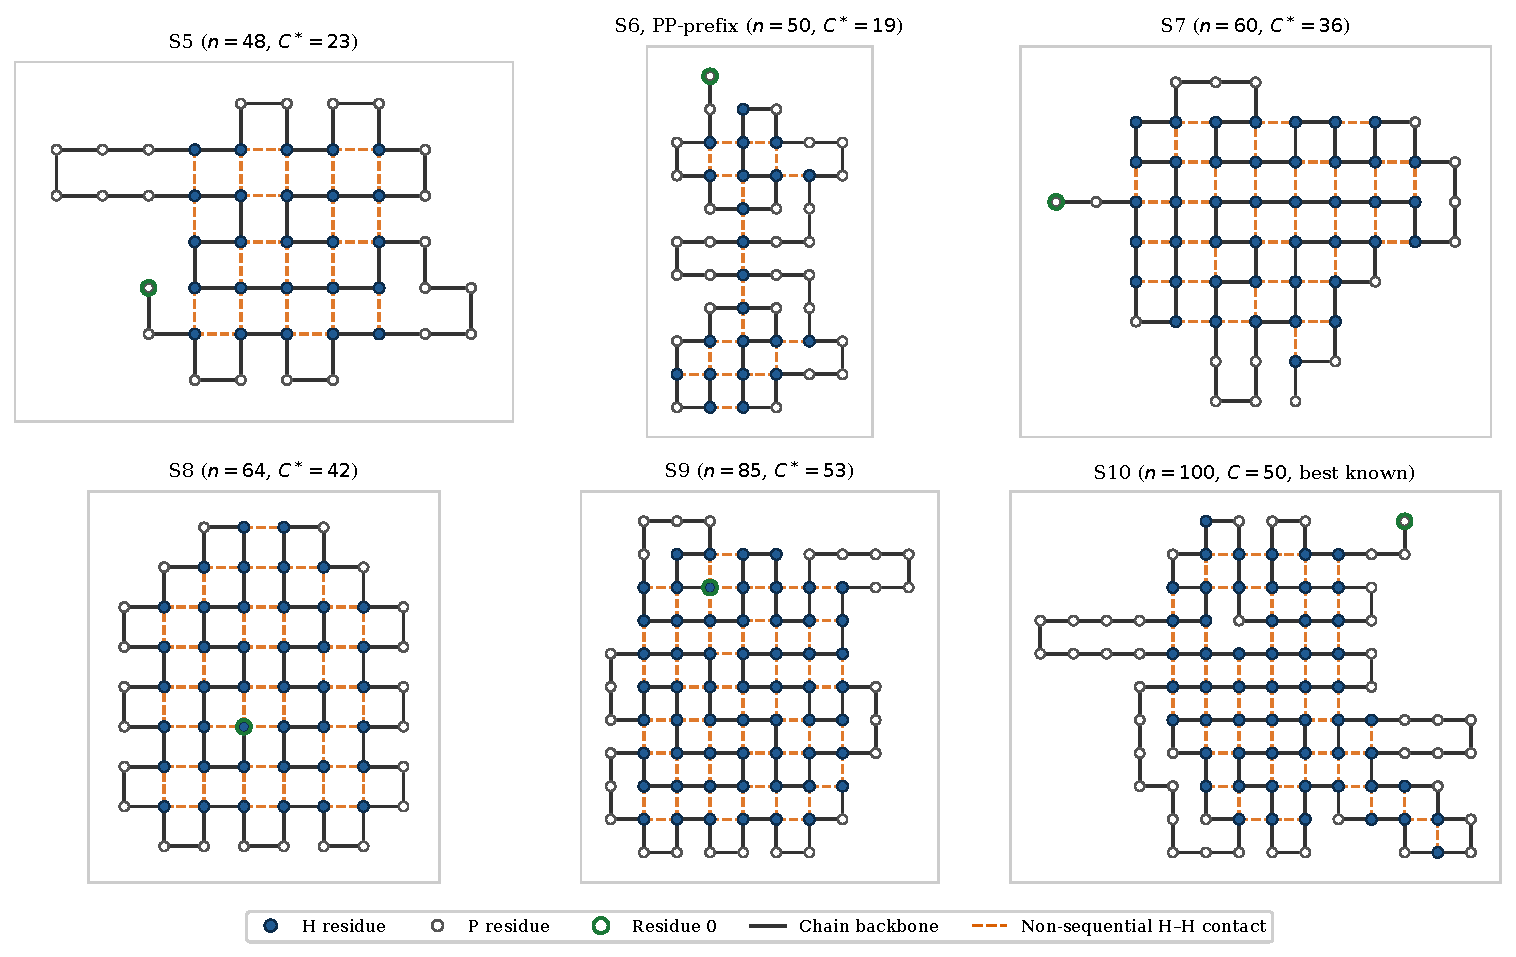
\includegraphics[width=\textwidth]{figures/fig1_optimal_folds_gallery.pdf}
\caption{Verified public lattice embeddings for S5, S6 (PP-prefix variant), and S7--S10. Filled dark circles denote H residues, open circles denote P residues, the green ring marks residue $0$, solid segments show the chain backbone, and dashed orange segments show non-sequential H--H contacts. S5, S6, S7, S8, and S9 are proven globally optimal over all of $\Z^2$ (Theorems~\ref{thm:opt} and~\ref{thm:s6}); a separate verified $21$-contact embedding for the canonical HH-prefix sequence \texttt{2D50} is archived in the companion repository.}
\label{fig:gallery}
\end{figure}

\section{Global Optimality for the PP-Prefix 50-Mer S6 on \texorpdfstring{$\Z^2$}{Z\string^2}}\label{sec:s6}

As shown in Table~\ref{tab:seqs}, the PP-prefix $50$-mer S6 ($n_H = 22$, $\mathrm{adj}_{HH} = 7$), printed in Chen and Huang~\cite[Table~1]{chen2005} with target contact count $21$, differs in its first four residues (\texttt{PPHP} versus \texttt{HHPH}) from Unger and Moult's~\cite{unger1993} canonical HH-prefix $50$-mer \texttt{2D50} ($n_H = 24$, $\mathrm{adj}_{HH} = 8$, proven optimal at $21$ in~\cite{giaquinta2013} and matched by our archived \texttt{2D50} fold). Combining Lemma~\ref{lem:spantree} with exact odd-H slack decomposition closes S6 unconditionally over all of $\Z^2$ with no artificial bounding-box restriction.

\begin{theorem}[Unconditional global optimality for PP-prefix S6 on $\Z^2$]\label{thm:s6}
For the PP-prefix sequence S6 ($n = 50$, $n_H = 22$, $\mathrm{adj}_{HH} = 7$), over all self-avoiding walks in $\Z^2$ (allowing connected or disconnected hydrophobic cores):
\begin{enumerate}[leftmargin=*,topsep=2pt,itemsep=1pt]
\item \emph{(Bipartite parity ceiling.)} $C(\mathrm{S6}) \le 21$, improving the Harary--Harborth bound of $27$ by $6$ contacts.
\item \emph{(Refutation of $C = 21$ and $C = 20$.)} No self-avoiding walk of S6 in $\Z^2$ achieves $C = 21$ or $C = 20$.
\item \emph{(Global optimum.)} $C^*(\mathrm{S6}) = 19$.
\end{enumerate}
\end{theorem}

\begin{proof}
\textbf{Part~(1).} S6 has $10$ odd-indexed H residues, $\{5, 7, 9, 11, 27, 31, 35, 37, 39, 49\}$, whose maximum H-core degrees are $(2, 2, 3, 4, 2, 2, 2, 3, 4, 4)$ (noting that endpoint $\mathrm{H}_{49}$ is adjacent to $\mathrm{H}_{48}$, so $d_{\max}(49) = 4$), summing to $28$, versus $12$ even-indexed H residues with degree sum $31$. Lemma~\ref{lem:parity} immediately gives $C(\mathrm{S6}) \le 28 - 7 = 21$.

\textbf{Part~(2): Soundness of Cuts~1--6.} We establish the validity of each modeling reduction used in the exact CP-SAT and pure-CNF formulations of Section~\ref{sec:formulations}:
\begin{enumerate}[label=\textbf{Cut~\arabic*.},leftmargin=*,topsep=2pt,itemsep=2pt]
\item \emph{Spanning-tree H-core diameter bound.} By Lemma~\ref{lem:spantree}(3), every fold $c \in (\Z^2)^{50}$ of S6 satisfies $\Delta_x(H) + \Delta_y(H) \le D$, where $D = 19$ for $C = 21$ and $D = 22$ for $C = 20$.
\item \emph{Rigid-motion symmetry breaking and exact finite diamond domains.} Applying a lattice rigid motion ($\Z^2 \rtimes D_4$) to any valid fold of S6 places the sequential H--H bond $(\mathrm{H}_{38}, \mathrm{H}_{39})$ at $p_0 = (0, 0)$ and $p_1 = (1, 0)$, and reflecting across $y = 0$ (which fixes $p_0$ and $p_1$ pointwise) enforces $y(c_{40}) \ge 0$ without loss of generality. Since $p_0, p_1 \in H$, every hydrophobic site $c_j \in H$ satisfies $\|c_j - p_0\|_1 \le \Delta_x(H) + \Delta_y(H) \le D$ and $\|c_j - p_1\|_1 \le D$. For any residue $i$ at chain distance $\mathrm{dist}_H(i) := \min_{s_j = \mathrm{H}} |i - j|$ from its nearest H residue, the triangle inequality along the chain yields
\[
  \|c_i - p_0\|_1 \le \min\bigl(|i - 38|,\; D + \mathrm{dist}_H(i)\bigr),
  \qquad
  \|c_i - p_1\|_1 \le \min\bigl(|i - 39|,\; D + \mathrm{dist}_H(i)\bigr),
\]
together with exact checkerboard parity $(x + y) \equiv i \pmod 2$. Restricting each residue $i$ to this finite diamond and enforcing $(x_{\max}(H) - x_{\min}(H)) + (y_{\max}(H) - y_{\min}(H)) \le D$ (with $x_{\min}(H) \le 0$, $x_{\max}(H) \ge 1$, $y_{\min}(H) \le 0$, $y_{\max}(H) \ge 0$ guaranteed by $p_0, p_1 \in H$) is therefore exact over all of $\Z^2$ without loss of generality.
\item \emph{Exact $\mathrm{P}_0, \mathrm{P}_1$ prefix relaxation.} Dropping the two leading polar residues $\mathrm{P}_0, \mathrm{P}_1$ and solving on the $48$-residue suffix $s_2 \dots s_{49}$ while retaining the full-sequence degree cap $d_{\max}(2) = 2$ for $\mathrm{H}_2$ (valid because in any $50$-mer embedding $\mathrm{P}_1$ and $\mathrm{P}_3$ occupy two distinct lattice neighbors of $\mathrm{H}_2$) removes only self-avoidance constraints and thus yields a relaxation (a superset of the feasible set).
\item \emph{Exact odd-H degree equations and exhaustive $10$-way case split.} For each odd H residue $i$, define its nonnegative slack $\sigma_i := d_{\max}(i) - \deg_H(c_i) \ge 0$. Since $\sum_{i \in \mathrm{Odd}(H)} \deg_H(c_i) = \mathrm{ie}(H) = C + 7$, we have $\sum_{i \in \mathrm{Odd}(H)} \sigma_i = 28 - (C + 7) = 21 - C$. Hence $C = 21$ forces $\sigma_i = 0$ for all $10$ odd H residues, whereas $C = 20$ forces $\sum \sigma_i = 1$, partitioning every $C = 20$ fold exhaustively into the $10$ subproblems $\sigma_k = 1$ and $\sigma_i = 0$ ($i \ne k$) for $k \in \{5, 7, 9, 11, 27, 31, 35, 37, 39, 49\}$.
\item \emph{Direct neighbor-forcing valid inequalities.} In the CP-SAT formulation, for each odd H residue $i \in \{11, 39, 49\}$ ($d_{\max} = 4$) and $i \in \{9, 37\}$ ($d_{\max} = 3$) with required H-core degree $r_i = d_{\max}(i) - \sigma_i$ in the current branch ($r_i = d_{\max}(i)$ at $C = 21$, and $r_i = d_{\max}(i) - \mathbf{1}_{i = k}$ in branch $k$ at $C = 20$), if residue $i$ occupies cell $u$ then Cut~4 requires $\sum_{v \in N(u)} z_{uv} = r_i$. Since $z_{uv} \le h_v$ for every neighbor $v \in N(u)$, at least $r_i$ neighbors of $u$ must satisfy $h_v = 1$ (in particular $p_{i,u} = 0$ if fewer than $r_i$ neighbors lie in the H-domain, and $p_{i,u} \le h_v$ for all $4$ neighbors when $r_i = 4$). These inequalities are direct logical consequences of Cut~4. (As noted in Section~\ref{sec:formulations}, the edge-free pure-CNF formulation enforces the corresponding neighborhood lower-bound clauses on all $10$ odd H residues.)
\item \emph{Relaxed H--H edge linearization.} Enforcing $z_{uv} \le h_u$ and $z_{uv} \le h_v$ without the reverse implication $z_{uv} \ge h_u + h_v - 1$ yields a relaxation (a superset of the feasible set) on $\sum z_{uv} = C + 7$ and is therefore sound for proving infeasibility.
\end{enumerate}
As detailed in Section~\ref{sec:verify} and Table~\ref{tab:s6cases}, the resulting $C = 21$ branch ($D = 19$) and all ten single-slack $C = 20$ branches ($D = 22$) are refuted independently by OR-Tools CP-SAT and CaDiCaL, with every CaDiCaL refutation checked by \texttt{lrat-check}, establishing Part~(2).

\textbf{Part~(3).} Combining Parts~(1) and~(2) gives $C^*(\mathrm{S6}) \le 19$, which is attained by the verified $19$-contact embedding in Figure~\ref{fig:gallery}.
\end{proof}

\section{Computational Verification and Benchmark Archive}\label{sec:verify}

\paragraph{Computing environment and software versions.}
All computations were executed on an Apple M3 Ultra workstation ($28$ CPU cores, $96\,$GiB unified memory, macOS) using Python~3.13.9, Google OR-Tools CP-SAT~9.15.6755~\cite{perron2023}, HiGHS~1.14.0~\cite{huangfu2018}, PicoSAT via \texttt{pycosat}~0.6.6~\cite{biere2008}, Z3~4.16.0~\cite{demoura2008}, CaDiCaL~3.1.0~\cite{biere2024}, and the unverified C reference clausal proof checkers \texttt{drat-trim}~\cite{wetzler2014} and \texttt{lrat-check} (implementing the LRAT format of~\cite{cruzfilipe2017}, as distinct from the formally verified Coq and ACL2 LRAT checkers introduced in~\cite{cruzfilipe2017} and CakeML's \texttt{cake\_lpr}~\cite{tan2021}). AI-assisted coding and editing tools were used during software implementation and manuscript preparation, as detailed in the Declarations section.

\paragraph{Multi-solver and DRAT verification for S7 and S8.}
For S8 ($6 \times 7$ rectangle, $\mathrm{pad} = 3$, two symmetric parity alignments of $6{,}188$ variables and $16{,}272$ clauses each; $12{,}376$ variables and $32{,}544$ clauses combined) and S7 (all four parity-compatible minimum-perimeter $43$-ominoes, $\mathrm{pad} = 5$, $8{,}700$--$8{,}729$ variables and $22{,}594$--$22{,}669$ clauses each), all four independent solvers report unsatisfiability (unless explicitly labeled solver-only, reported times are end-to-end Python wall-clock times covering model/CNF construction and solving):
\begin{itemize}[leftmargin=*,topsep=2pt,itemsep=1pt]
\item \emph{OR-Tools CP-SAT:} $0.03\,$s for S8 and $0.16\,$s total for S7 ($0.19\,$s combined, including Ferrers polyomino enumeration, parity filtering, model construction, and solving).
\item \emph{HiGHS MILP:} $0.12\,$s for S8 and $0.33\,$s total for S7 ($0.45\,$s combined for MILP construction and solving, excluding the ${\sim}0.05\,$s S7 Ferrers enumeration step).
\item \emph{PicoSAT pure CNF:} $0.027\,$s for S8 and $0.065\,$s total for S7 ($0.092\,$s combined for CNF construction and solving; pure \texttt{pycosat.solve} solver-only time is $0.007\,$s for S8 and $0.020\,$s for S7, or $0.027\,$s combined).
\item \emph{Z3 DRAT emission and independent checking:} Solving all six instances in $0.91\,$s of Z3 solver-only (\texttt{s.check()}) time ($0.37\,$s for S8 and $0.54\,$s for S7; end-to-end Python wall time is $5.98\,$s, dominated by $4.84\,$s for constructing the $123{,}097$ Z3 clause AST objects via the Python bindings plus $0.17\,$s for proof-tree extraction), Z3 generates standard DRAT/RUP refutations of $23$ and $12$ clauses for S8 ($639$ and $114\,$B) and $8, 9, 12$, and $10$ clauses for S7 ($57, 109, 234$, and $156\,$B; $1{,}309\,$B across all six certificates). Each certificate is checked by \texttt{drat-trim} in $0.024$--$0.027\,$s ($0.15\,$s total) and by a compact pure-Python RUP checker using only the Python standard library in $0.18\,$s for S8 and $0.34\,$s for S7, or $0.58\,$s end-to-end including $0.06\,$s for four-corner Ferrers polyomino enumeration and setup.
\end{itemize}

\paragraph{Feasibility sanity checks and dual-solver LRAT verification for S6.}
To guard against modeling over-constraint, we test the same CP-SAT and pure-CNF encodings used for the S6 refutations at $C = 19$ with odd-H slack set $\{31, 37\}$ (matching the two unit odd-H slacks of our archived $19$-contact fold) and $D = 19$. OR-Tools CP-SAT ($4$ workers) returns a feasible solution in $26.51\,$s ($82{,}095$ conflicts), and CaDiCaL~3.1.0 returns satisfiable in $15.82\,$s on the pure-CNF encoding ($29{,}426$ variables, $90{,}528$ clauses); both extract directly verified $19$-contact self-avoiding walks of $s_2 \dots s_{49}$. Independently, rather than searching from scratch, HiGHS MILP ($0.35\,$s) and PicoSAT ($0.053\,$s, zero violated clauses across $90{,}528$ clauses) evaluate the \emph{fixed} rigidly aligned archived $50$-mer fold for S6 inside the $D = 19$ encoding (fixing its $48$ suffix placements as unit constraints or assumptions, so PicoSAT resolves the remaining auxiliary variables essentially by unit propagation in $0.053\,$s), confirming that the archived embedding (which satisfies $\Delta_x(H) + \Delta_y(H) = 13 \le 19$) obeys every constraint of the unconditional $\Z^2$ formulation.

Across the eleven unsatisfiable branches ($C = 21$ with $29{,}426$ variables and $90{,}728$ clauses; ten $C = 20$ single-slack branches with $35{,}395$ variables and $108{,}979$--$111{,}226$ clauses), Table~\ref{tab:s6cases} and Figure~\ref{fig:bounds}(b) report the complete dual-solver and \texttt{lrat-check} verification ledger. OR-Tools CP-SAT ($6$ workers per branch) refutes $C = 21$ in $45.75\,$s and all ten $C = 20$ branches in $1013.95\,$s cumulative ($1059.70\,$s total). CaDiCaL~3.1.0 (single-threaded per branch, emitting uncompressed LRAT proofs) refutes $C = 21$ in $96.95\,$s ($3.44\,$GB) and all ten $C = 20$ branches in $1699.66\,$s cumulative ($61.48\,$GB), totaling $1796.61\,$s and $64.92\,$GB ($60.46\,$GiB). Every LRAT proof is checked by \texttt{lrat-check} in $36.32\,$s for $C = 21$ and $660.43\,$s cumulative across the ten $C = 20$ branches ($696.75\,$s total).

\begin{table}[t]
\centering
\caption{Unconditional $\Z^2$ dual-solver and \texttt{lrat-check} proof ledger for S6. Every unsatisfiable branch is refuted independently by OR-Tools CP-SAT ($6$ workers; $4$ for the $C = 19$ sanity check) and CaDiCaL~3.1.0 ($1$ thread per branch) with an LRAT proof checked by \texttt{lrat-check}.}
\label{tab:s6cases}
\scriptsize
\setlength{\tabcolsep}{5pt}
\begin{tabular}{@{}lrrrrrrr@{}}
\toprule
\textbf{Branch} & \textbf{$C$} & \textbf{Slack} & \textbf{$D$} & \textbf{CP-SAT (s)} & \textbf{CaDiCaL (s)} & \textbf{LRAT (GB)$^{\dagger}$} & \textbf{\texttt{lrat-check} (s)} \\
\midrule
Sanity check & $19$ & $\{31, 37\}$ & $19$ & $26.51$ (SAT) & $15.82$ (SAT) & --- & $19$-contact SAW \\
\midrule
Uncond.\ $C = 21$ & $21$ & $\emptyset$ & $19$ & $45.75$ & $96.95$ & $3.44$ & $36.32$ (checked) \\
\midrule
$C = 20$, $k = \mathrm{H}_5$ & $20$ & $\{5\}$ & $22$ & $54.33$ & $114.15$ & $4.00$ & $43.00$ (checked) \\
$C = 20$, $k = \mathrm{H}_7$ & $20$ & $\{7\}$ & $22$ & $57.74$ & $86.24$ & $2.94$ & $31.49$ (checked) \\
$C = 20$, $k = \mathrm{H}_9$ & $20$ & $\{9\}$ & $22$ & $64.27$ & $133.69$ & $4.75$ & $50.96$ (checked) \\
$C = 20$, $k = \mathrm{H}_{11}$ & $20$ & $\{11\}$ & $22$ & $107.73$ & $180.37$ & $6.54$ & $70.33$ (checked) \\
$C = 20$, $k = \mathrm{H}_{27}$ & $20$ & $\{27\}$ & $22$ & $61.90$ & $100.76$ & $3.56$ & $38.62$ (checked) \\
$C = 20$, $k = \mathrm{H}_{31}$ & $20$ & $\{31\}$ & $22$ & $57.78$ & $119.93$ & $4.33$ & $46.20$ (checked) \\
$C = 20$, $k = \mathrm{H}_{35}$ & $20$ & $\{35\}$ & $22$ & $111.64$ & $179.01$ & $6.59$ & $71.36$ (checked) \\
$C = 20$, $k = \mathrm{H}_{37}$ & $20$ & $\{37\}$ & $22$ & $176.36$ & $260.76$ & $10.00$ & $107.30$ (checked) \\
$C = 20$, $k = \mathrm{H}_{39}$ & $20$ & $\{39\}$ & $22$ & $219.37$ & $389.42$ & $13.80$ & $147.57$ (checked) \\
$C = 20$, $k = \mathrm{H}_{49}$ & $20$ & $\{49\}$ & $22$ & $102.83$ & $135.33$ & $4.96$ & $53.60$ (checked) \\
\midrule
\textbf{$C = 20$ subtotal} & $20$ & all $10$ & $22$ & $1013.95$ & $1699.66$ & $61.48$ & $660.43$ (10 checked) \\
\textbf{All UNSAT total} & $\ge 20$ & all $11$ & $19/22$ & $1059.70$ & $1796.61$ & $64.92$ & $696.75$ (11 checked) \\
\bottomrule
\end{tabular}
\par\vspace{2pt}
\begin{minipage}{\textwidth}
\scriptsize $^{\dagger}$LRAT sizes are reported in decimal gigabytes ($1\,\mathrm{GB} = 10^9\,$B); individual $C = 20$ entries rounded to two decimal places sum to $61.47\,$GB, whereas the exact sum is $61.4817\,$GB ($57.26\,$GiB), and $64.9177\,$GB ($60.46\,$GiB) including $C = 21$. CaDiCaL and \texttt{lrat-check} times are cumulative single-thread runtimes across branches.
\end{minipage}
\end{table}

\begin{figure}[tb]
\centering
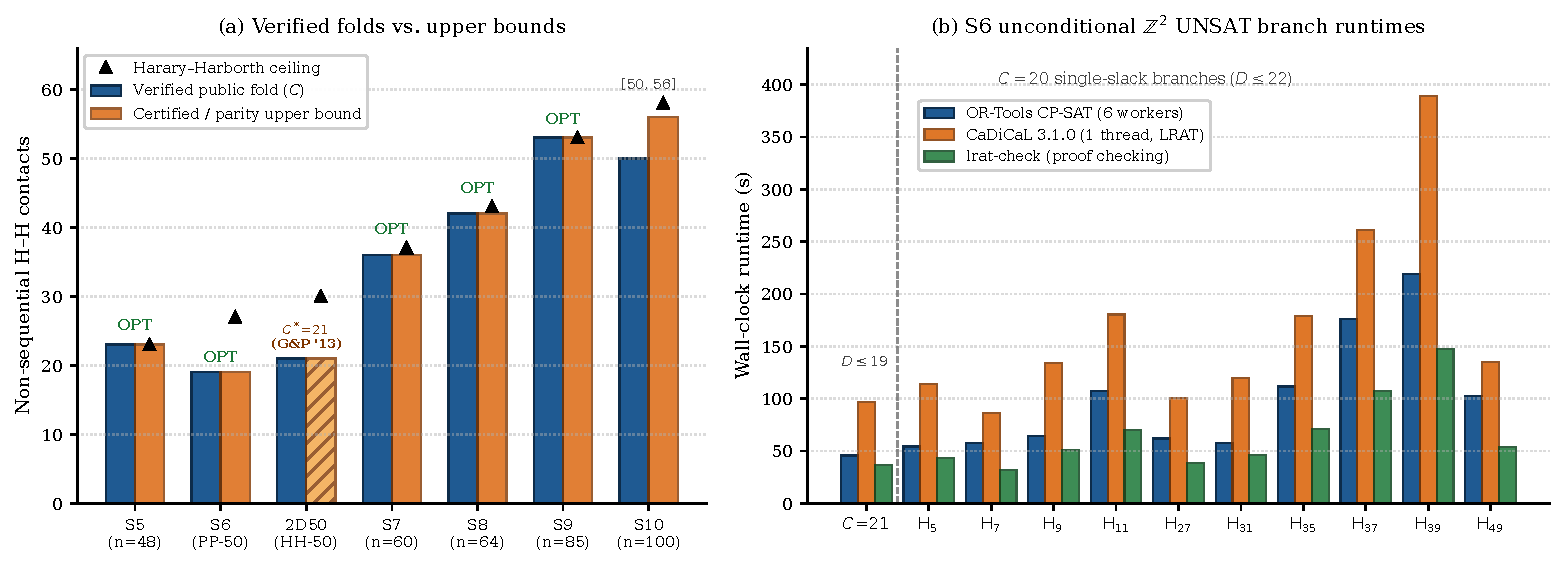
\includegraphics[width=\textwidth]{figures/fig2_optimality_bounds_and_s6.pdf}
\caption{Optimality bounds across S5, S6 (PP-prefix variant), \texttt{2D50}, and S7--S10, together with S6 branch runtimes. (a)~Verified public contact counts against the tightest known upper bounds and Harary--Harborth ceilings; S5, S6, S7, S8, and S9 are certified optimal on $\Z^2$ in this work, \texttt{2D50} matches the exact optimum $C^* = 21$ of~\cite{giaquinta2013} (hatched bar; our analytic parity bound is $25$), and S10 retains the open interval $[50, 56]$. (b)~Wall-clock runtimes for OR-Tools CP-SAT, CaDiCaL~3.1.0, and \texttt{lrat-check} across all eleven unsatisfiable S6 branches on $\Z^2$ (Table~\ref{tab:s6cases}).}
\label{fig:bounds}
\end{figure}

Table~\ref{tab:summary} summarizes the achieved contact counts, analytic upper bounds, and global optimality status across all seven benchmark sequences. The archived lower-bound embeddings for S5--S9 and \texttt{2D50} were generated using our repository's hybrid Monte Carlo and constraint-routing routines---combining simulated annealing and Wang--Landau/replica-exchange search, spatial-window CP-SAT large neighborhood search, and target H-core CP-SAT routability (for example, S5 via $5\times 5$ H-core routing, S9 via CP-SAT routability on a one-cell H-core modification of a $52$-contact fold, and \texttt{2D50} via multi-chain simulated annealing)---and are certified directly by the standalone coordinate verifier independently of their generation history. For the open $100$-mer S10 (\texttt{2D100b}), the archived $50$-contact conformation matches the best reported literature value of $C = 50$~\cite{hsu2003,wust2012,zhang2007} and was obtained using our crossover genetic algorithm (archived in the companion repository; see Data and Code Availability), which combines contact-weighted parent selection from an elite pool, single-point prefix--suffix splicing tested across all $D_4$ lattice isometries and adjacent attachment sites to preserve self-avoidance, occasional macro-move mutations, and greedy local polishing with pull, pivot, corner-flip, crankshaft, and rebridging moves.

\begin{table}[tb]
\centering
\caption{Benchmark summary across S5, S6 (PP-prefix variant), \texttt{2D50}, and S7--S10. All archived coordinate embeddings pass automated self-avoidance, adjacency, and contact-count verification.}
\label{tab:summary}
\footnotesize
\begin{tabular}{@{}lrrrrrrl@{}}
\toprule
\textbf{Seq} & $n$ & $n_H$ & $\mathrm{adj}_{HH}$ & \textbf{HH} & \textbf{Par.} & \textbf{$C$} & \textbf{Unconditional $\Z^2$ Optimality Status} \\
\midrule
S5 & 48 & 25 & 17 & 23 & 25 & \textbf{23} & \textbf{Proven optimal on $\Z^2$} (Harary--Harborth; confirms~\cite{giaquinta2013}) \\
S6 & 50 & 22 & 7 & 27 & 21 & \textbf{19} & \textbf{Proven optimal on $\Z^2$} (PP-prefix~\cite{chen2005}; CP-SAT + LRAT) \\
\texttt{2D50} & 50 & 24 & 8 & 30 & 25 & \textbf{21} & Matches canonical optimum~\cite{giaquinta2013} (HH-prefix~\cite{unger1993}) \\
S7 & 60 & 43 & 35 & 37 & 40 & \textbf{36} & \textbf{Proven optimal on $\Z^2$} (4 solvers + DRAT; confirms~\cite{giaquinta2013}) \\
S8 & 64 & 42 & 28 & 43 & 43 & \textbf{42} & \textbf{Proven optimal on $\Z^2$} (4 solvers + DRAT; confirms~\cite{giaquinta2013}) \\
S9 & 85 & 59 & 49 & 53 & 58 & \textbf{53} & \textbf{Proven optimal on $\Z^2$} (Harary--Harborth; confirms~\cite{giaquinta2013}) \\
S10 & 100 & 56 & 39 & 58 & 56 & \textbf{50} & Matches record~\cite{hsu2003,wust2012,zhang2007} (crossover GA; open) \\
\bottomrule
\end{tabular}
\end{table}

\section{Conclusion, Limitations, and Trusted Computing Base}\label{sec:conclusion}

We have established unconditional global optimality on $\Z^2$ for S5 ($C^* = 23$) and S9 ($C^* = 53$) analytically via the one-line Harary--Harborth isoperimetric upper bound, and for S7 ($C^* = 36$) and S8 ($C^* = 42$) across four independent solvers (OR-Tools CP-SAT, HiGHS MILP, PicoSAT, and Z3) backed by six archived DRAT refutation proofs checked by \texttt{drat-trim} and a standalone pure-Python RUP checker. We further introduced an exact spanning-tree H-core diameter bound valid for disconnected hydrophobic cores, paired with small-component bounds under at most one unit of parity degree slack (Lemma~\ref{lem:spantree}), resolved the published $n = 50$ benchmark discrepancy from Chen and Huang~\cite[Table~1]{chen2005} by certifying $C^*(\mathrm{S6}) = 19$ unconditionally alongside a verified $21$-contact fold for \texttt{2D50}, and archived machine-verified public coordinates for all seven benchmarks.

\paragraph{Trusted computing base (TCB).}
Every computational unsatisfiability result in Theorems~\ref{thm:opt} and~\ref{thm:s6} is backed by independent clausal proof checking (DRAT/LRAT), removing the search engines (OR-Tools CP-SAT, HiGHS, PicoSAT, Z3, and CaDiCaL) from the trust chain for UNSAT claims. The remaining TCB consists of four compact components: (i)~the Python CNF generators translating the formulations of Section~\ref{sec:formulations} into DIMACS CNF (validated against over-constraint by the $C = 19$ feasibility sanity checks across all four solvers); (ii)~the unverified C reference clausal proof checkers \texttt{drat-trim}~\cite{wetzler2014} and \texttt{lrat-check} (implementing the LRAT format of~\cite{cruzfilipe2017}, distinct from the formally verified Coq and ACL2 LRAT checkers introduced in~\cite{cruzfilipe2017} and CakeML's \texttt{cake\_lpr}~\cite{tan2021}; supplemented by our pure-Python RUP checker for S7 and S8, while the generated standard LRAT traces remain amenable to drop-in re-checking by any formally verified LRAT checker); (iii)~the four-corner Ferrers polyomino enumerator and parity filter for S7 (and the integer-partition verifier for Lemma~\ref{lem:spantree}); and (iv)~the coordinate verifier confirming self-avoidance, adjacency, and contact counts for lower-bound folds.

\paragraph{Proof artifact archival and reproducibility.}
For S7 and S8, all six DRAT files ($1{,}309\,$B total) are archived directly in the repository and re-checked in under $0.6\,$s. For S6, the eleven uncompressed LRAT traces total $64.92\,$GB ($60.46\,$GiB, where $1\,\mathrm{GB} = 10^9\,$B) and are deleted after checking rather than committed; the pipeline regenerates and re-checks all eleven proofs in approximately $42\,$min of cumulative single-thread CPU time (roughly $15$--$20\,$min wall time on three parallel workers). Exact SHA-256 digests of every DIMACS CNF and LRAT file are archived as run-verification checksums (CNF digests are platform-independent; LRAT digests correspond to CaDiCaL~3.1.0).

\paragraph{Limitations and future work.}
Lemma~\ref{lem:spantree} is sharpest when the gap between the bipartite parity upper bound and the target contact count leaves minimal parity slack ($s_{\min} \le 1$). For the canonical HH-prefix sequence \texttt{2D50} (parity bound $25$, exact optimum $21$~\cite{giaquinta2013}), refuting $C = 22$ entails $s_{\min} = 3$, which allows isolated singletons and pairs of both parities and expands the number of slack-distribution branches substantially. Similarly, closing the $[50, 56]$ gap on the $100$-mer S10 ($n_H = 56$, $\mathrm{adj}_{HH} = 39$, parity bound $56$, Harary--Harborth bound $58$) requires either tighter local degree cuts or larger symmetry-reduced case decompositions and remains open. Extending certified clausal proof pipelines to higher-slack 2D instances and 3D cubic or face-centered-cubic benchmarks is a natural direction for future research.

\section*{Declarations}

\paragraph{Funding.} This research received no external funding.

\paragraph{Competing Interests.} The author declares no competing interests.

\paragraph{Data and Code Availability.}
All verified coordinate files, exact optimality and proof-generation scripts, crossover genetic algorithm and heuristic search routines (including \path{src/hp_folding/crossover_ga.py}), archived DRAT certificates for S7 and S8, S6 JSON verification ledgers and SHA-256 digests, figure scripts, and automated tests are archived at tagged release \texttt{v1.0.0} (\url{https://github.com/Brsanch/hp-folding/releases/tag/v1.0.0}; repository root \url{https://github.com/Brsanch/hp-folding}) under the Apache-2.0 license (\texttt{LICENSE}).

\paragraph{Declaration of AI-Assisted Tools.}
Large language models (Anthropic Claude and Google Gemini) were used during algorithm prototyping, software implementation, exposition drafting, and manuscript editing. Every combinatorial lemma, solver encoding, archived DRAT proof, and checked LRAT certificate was reviewed, executed, and verified by the author. All figures were generated programmatically from verified coordinate and solver-log data; no generative AI imagery was used. The author assumes full responsibility for all content.

\begin{thebibliography}{32}

\bibitem{backofen2006}
R.~Backofen and S.~Will.
A constraint-based approach to fast and exact structure prediction in three-dimensional protein models.
\emph{Constraints}, 11(1):5--30, 2006.

\bibitem{bastolla1998}
U.~Bastolla, H.~Frauenkron, E.~Gerstner, P.~Grassberger, and W.~Nadler.
Testing a new Monte Carlo algorithm for protein folding.
\emph{Proteins}, 32(1):52--66, 1998.

\bibitem{berger1998}
B.~Berger and T.~Leighton.
Protein folding in the hydrophobic-hydrophilic (HP) model is NP-complete.
\emph{J.\ Comput.\ Biol.}, 5(1):27--40, 1998.

\bibitem{beutler1996}
T.~C.~Beutler and K.~A.~Dill.
A fast conformational search strategy for finding low energy structures of model proteins.
\emph{Protein Sci.}, 5(10):2037--2043, 1996.

\bibitem{biere2008}
A.~Biere.
PicoSAT essentials.
\emph{J.\ Satisf.\ Boolean Model.\ Comput.}, 4(2--4):75--97, 2008.

\bibitem{biere2024}
A.~Biere, T.~Faller, K.~Fazekas, M.~Fleury, N.~Froleyks, and F.~Pollitt.
CaDiCaL~2.0.
In \emph{Computer Aided Verification (CAV~2024)}, Lecture Notes in Computer Science, vol.~14681, pp.~133--152. Springer, 2024. (Version~3.1.0 used here.)

\bibitem{chen2005}
M.~Chen and W.~Q.~Huang.
A branch and bound algorithm for the protein folding problem in the HP lattice model.
\emph{Genomics Proteomics Bioinformatics}, 3(4):225--230, 2005.

\bibitem{crescenzi1998}
P.~Crescenzi, D.~Goldman, C.~Papadimitriou, A.~Piccolboni, and M.~Yannakakis.
On the complexity of protein folding.
\emph{J.\ Comput.\ Biol.}, 5(3):423--465, 1998.

\bibitem{cruzfilipe2017}
L.~Cruz-Filipe, M.~J.~H.~Heule, W.~A.~Hunt, Jr., M.~Kaufmann, and P.~Schneider-Kamp.
Efficient certified RAT verification.
In \emph{Automated Deduction (CADE-26)}, Lecture Notes in Computer Science, vol.~10395, pp.~220--236. Springer, 2017.

\bibitem{davis2016}
L.~K.~Davis.
A parallel trajectory swapping Wang--Landau study of the HP protein model.
Master's thesis, Swansea University, \texttt{arXiv:1607.03253}, 2016.

\bibitem{demoura2008}
L.~de~Moura and N.~Bj{\o}rner.
Z3: An efficient SMT solver.
In \emph{Tools and Algorithms for the Construction and Analysis of Systems (TACAS~2008)}, Lecture Notes in Computer Science, vol.~4963, pp.~337--340. Springer, 2008.

\bibitem{dill1985}
K.~A.~Dill.
Theory for the folding and stability of globular proteins.
\emph{Biochemistry}, 24(6):1501--1509, 1985.

\bibitem{dotu2011}
I.~Dot\'u, M.~Cebri\'an, P.~Van~Hentenryck, and P.~Clote.
On lattice protein structure prediction revisited.
\emph{IEEE/ACM Trans.\ Comput.\ Biol.\ Bioinform.}, 8(6):1620--1632, 2011.

\bibitem{giaquinta2013}
E.~Giaquinta and L.~Pozzi.
An effective exact algorithm and a new upper bound for the number of contacts in the hydrophobic-polar two-dimensional lattice model.
\emph{J.\ Comput.\ Biol.}, 20(8):593--609, 2013.

\bibitem{harary1976}
F.~Harary and H.~Harborth.
Extremal animals.
\emph{J.\ Combin.\ Inform.\ System Sci.}, 1(1):1--8, 1976.

\bibitem{hart1996}
W.~E.~Hart and S.~Istrail.
Fast protein folding in the hydrophobic-hydrophilic model within three-eighths of optimal.
\emph{J.\ Comput.\ Biol.}, 3(1):53--96, 1996.

\bibitem{hsu2003}
H.-P.~Hsu, V.~Mehra, W.~Nadler, and P.~Grassberger.
Growth algorithms for lattice heteropolymers at low temperatures.
\emph{J.\ Chem.\ Phys.}, 118(1):444--451, 2003.

\bibitem{huangfu2018}
Q.~Huangfu and J.~A.~J.~Hall.
Parallelizing the dual revised simplex method.
\emph{Math.\ Program.\ Comput.}, 10(1):119--142, 2018.

\bibitem{lau1989}
K.~F.~Lau and K.~A.~Dill.
A lattice statistical mechanics model of the conformational and sequence spaces of proteins.
\emph{Macromolecules}, 22(10):3986--3997, 1989.

\bibitem{liang2001}
F.~Liang and W.~H.~Wong.
Evolutionary Monte Carlo for protein folding simulations.
\emph{J.\ Chem.\ Phys.}, 115(7):3374--3380, 2001.

\bibitem{mann2008}
M.~Mann, S.~Will, and R.~Backofen.
CPSP-tools---Exact and complete algorithms for high-throughput 3D lattice protein studies.
\emph{BMC Bioinformatics}, 9:230, 2008.

\bibitem{newman2002}
A.~Newman.
A new algorithm for protein folding in the HP model.
In \emph{Proceedings of the Thirteenth Annual ACM--SIAM Symposium on Discrete Algorithms (SODA~2002)}, pp.~876--884. SIAM, 2002.

\bibitem{perron2023}
L.~Perron, F.~Didier, and S.~Gay.
The CP-SAT-LP solver.
In \emph{29th International Conference on Principles and Practice of Constraint Programming (CP~2023)}, LIPIcs, vol.~280, pp.~3:1--3:2. Schloss Dagstuhl, 2023. (Google OR-Tools CP-SAT v9.15.6755.)

\bibitem{ramakrishnan1997}
R.~Ramakrishnan, B.~Ramachandran, and J.~F.~Pekny.
A dynamic Monte Carlo algorithm for exploration of dense conformational spaces in heteropolymers.
\emph{J.\ Chem.\ Phys.}, 106(6):2418--2425, 1997.

\bibitem{sinz2005}
C.~Sinz.
Towards an optimal CNF encoding of boolean cardinality constraints.
In \emph{Principles and Practice of Constraint Programming (CP~2005)}, Lecture Notes in Computer Science, vol.~3709, pp.~827--831. Springer, 2005.

\bibitem{tan2021}
Y.~K.~Tan, M.~J.~H.~Heule, and M.~O.~Myreen.
\texttt{cake\_lpr}: Verified propagation redundancy checking in CakeML.
In \emph{Tools and Algorithms for the Construction and Analysis of Systems (TACAS~2021)}, Lecture Notes in Computer Science, vol.~12652, pp.~223--241. Springer, 2021.

\bibitem{unger1993}
R.~Unger and J.~Moult.
Genetic algorithms for protein folding simulations.
\emph{J.\ Mol.\ Biol.}, 231(1):75--81, 1993.

\bibitem{wetzler2014}
N.~Wetzler, M.~J.~H.~Heule, and W.~A.~Hunt, Jr.
DRAT-trim: Efficient checking and trimming using expressive clausal proofs.
In \emph{Theory and Applications of Satisfiability Testing (SAT~2014)}, Lecture Notes in Computer Science, vol.~8561, pp.~422--429. Springer, 2014.

\bibitem{will2002}
S.~Will.
Constraint-based hydrophobic core construction for protein structure prediction in the face-centered-cubic lattice.
In \emph{Pacific Symposium on Biocomputing (PSB~2002)}, pp.~661--672. World Scientific, 2002.

\bibitem{wust2012}
T.~W\"ust and D.~P.~Landau.
Optimized Wang--Landau sampling of lattice polymers: Ground state search and folding thermodynamics of HP model proteins.
\emph{J.\ Chem.\ Phys.}, 137(6):064903, 2012.

\bibitem{yanev2017}
N.~Yanev, M.~Traykov, P.~Milanov, and B.~Yurukov.
Protein folding prediction in a cubic lattice in hydrophobic-polar model.
\emph{J.\ Comput.\ Biol.}, 24(5):412--421, 2017.

\bibitem{yue1995}
K.~Yue and K.~A.~Dill.
Forces of tertiary structural organization in globular proteins.
\emph{Proc.\ Natl.\ Acad.\ Sci.\ USA}, 92(1):146--150, 1995.

\bibitem{zhang2007}
J.~Zhang, S.~C.~Kou, and J.~S.~Liu.
Biopolymer structure simulation and optimization via fragment regrowth Monte Carlo.
\emph{J.\ Chem.\ Phys.}, 126(22):225101, 2007.

\end{thebibliography}

\end{document}
